\documentclass{article}

% Language setting
% Replace `english' with e.g. `spanish' to change the document language
\usepackage[english]{babel}

% Set page size and margins
% Replace `letterpaper' with `a4paper' for UK/EU standard size
\usepackage[letterpaper,top=2cm,bottom=2cm,left=3cm,right=3cm,marginparwidth=1.75cm]{geometry}

% Useful packages
\usepackage{amsmath}
\usepackage{graphicx}
\usepackage[colorlinks=true, allcolors=blue]{hyperref}
\usepackage{tabularx}

\title{\textbf{LLM Prompt Strategies for Commonsense-Reasoning Tasks}
}
\author{Tesa Robič, Tim Dolenc, Matjaž Bevc}

\begin{document}
\maketitle


\section{Introduction}

In this project we will research, compare and evaluate different prompt strategies for commonsense reasoning tasks used in Large Language Models (LLM). LLMs are really good at understanding and generating text. But when it comes to understanding common sense (the things we know about the world without being told), they need help. So, researchers are trying out different ways to give these models hints or instructions, called prompts. There are many different prompt strategies like Chain Of Thought (CoT), In-Context Learning (ICL), plan-and-solve techniques, Tree Of Thought, Retrieval augmentation (RAG) and more. In the next chapter, we introduce different strategies that we consider using for this project [1].


\section{Existing solutions and Realated Work}
\subsection{Chain-of-Thought (CoT) prompting}

Chain-of-thought prompting enables large language models to tackle complex arithmetic, commonsense, and symbolic reasoning tasks. CoT prompting involves providing intermediate reasoning steps to guide the model’s responses, which can be facilitated through simple prompts such as “Let’s think step by step” or through a series of manual demonstrations, each composed of a question and a reasoning chain that leads to an answer [1].

\begin{center}
    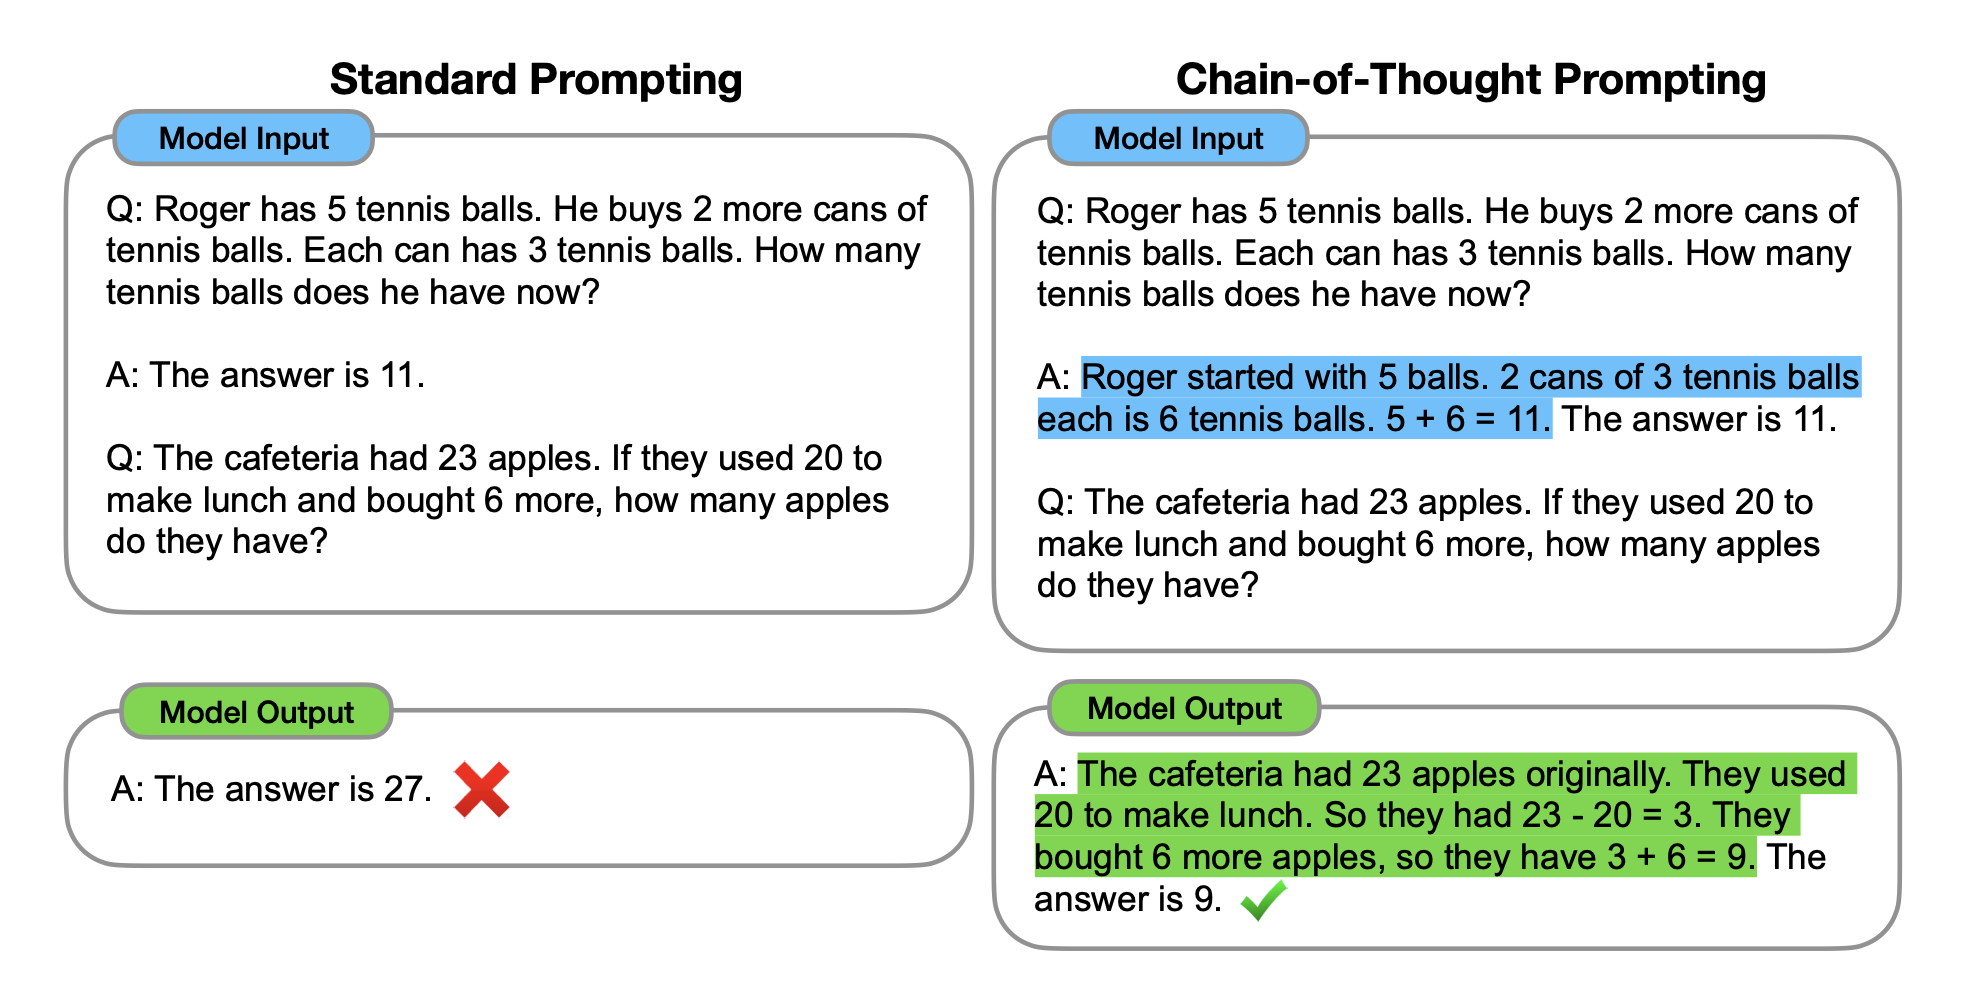
\includegraphics[scale=0.45]{Screenshot 2024-03-21 at 10.21.03.png}
    Figure 1: An illustration of standard LLM prompting on the left, and chain-of-thought prompting on the right.
\end{center}

Some benefits of CoT promting:
\begin{itemize}
    \item \textbf{Improved accuracy}: With clear reasoning steps, the LLM is less likely to make mistakes or jump to illogical conclusions. This is especially helpful for tasks with multi-step logic or complex reasoning requirements.
    \item \textbf{Transparency:} CoT prompts make the reasoning process more transparent, allowing us to understand how the LLM arrived at its answer. This is crucial for building trust and identifying potential bias or errors.
    \item \textbf{Better performance on complex tasks:} CoT is particularly effective for tasks that require multi-step reasoning, logical deduction or \textit{common-sense} application. These are areas where past LLMs often struggled.
    \item \textbf{Adaptability}: The technique can be used for various tasks, from solving math problems and interpreting data to summarizing text and even creative writing.
    \item \textbf{Precision-Guided Reasoning:} By providing a clear path, CoT reduces the risk of LLMs stumbling into erroneous conclusions or leaps of illogical faith. Multi-step tasks and convoluted reasoning problems, once impenetrable to LLMs, become navigable landscapes with CoT at the helm.

\end{itemize}

Limitations of CoT prompting:
\begin{itemize}
    \item \textbf{Manual effort:} Creating effective CoT prompts requires understanding the problem and designing the reasoning steps yourself. This can be time-consuming and complex for intricate tasks.
    \item \textbf{Model size:} CoT seems to be more effective for larger LLMs with stronger reasoning capabilities. Smaller models might struggle to follow the prompts or generate their own reasoning chains.
    \item \textbf{Prompt bias:} Like any other prompting technique, CoT can be susceptible to biased prompts that lead the LLM to incorrect conclusions. Careful design and testing are crucial.
    \item \textbf{Bias Blind Spots:} Just like any prompt, CoT is susceptible to biased information. Careful design and thorough testing are crucial to ensure the LLM doesn’t follow a misleading path
    \item \textbf{Crafting the Path:} Building effective CoT prompts requires understanding the problem’s intricacies and formulating a clear, logical chain of reasoning. This can be demanding, especially for complex tasks. [6]

\end{itemize}

\subsubsection{Auto CoT}
When applying chain-of-thought prompting with demonstrations, the process involves hand-crafting effective and diverse examples. This manual effort could lead to suboptimal solutions. Zhang et al. [2] propose an approach to eliminate manual efforts by leveraging LLMs with "Let's think step by step" prompt to generate reasoning chains for demonstrations one by one. This automatic process can still end up with mistakes in generated chains. To mitigate the effects of the mistakes, the diversity of demonstrations matter. This work proposes Auto-CoT, which samples questions with diversity and generates reasoning chains to construct the demonstrations [3]. 

\subsection{In-context Learning (ICL)}

The key idea of in-context learning is to learn from analogy. Figure below shows how ICL works. First ICL requires a few examples to form a demonstration context. These examples are usually written in natural language templates. Then it concatenates a query question and a piece of demonstration context together to form a prompt which is then fed into the language model for prediction [4]. 

\begin{center}
    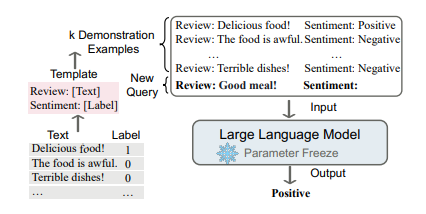
\includegraphics[]{icl.png}
    Figure 2: ICL demonstration
\end{center}
In-context learning is a method that helps models understand information better by giving them context right in the question. Instead of just asking a question on its own, in-context learning adds extra details or examples to help the model understand what's being asked. For example, instead of asking "What is a cat?" in isolation, in-context learning might say "Imagine you see a fluffy animal with pointy ears and whiskers. What do you think it is?" By providing context within the question itself, in-context learning helps models make better sense of the information and give more accurate answers [4] [5].

\subsection{Plan-and-Solve (PS) prompting}
With Zero-shot CoT, there are three pitfalls: calculation errors, missing-reasoning-step errors and semantic understanding errors. 

The first two pitfalls can be addressed with Plan-and-Solve prompting (PS and PS+).
\newline

Plan-and-Solve prompting consists of two components: devising a plan to divide the task into small subtasks and carrying out the subtasks according to the plan. While Zero-Shot CoT appends the phrase \textit{"Let's think step by step"} to the prompt, PS appends \textit{"Let’s first understand theproblem and devise a plan to solve the problem. Then, let’s carry out the plan and solve the problem step by step." }
\newline

Extending the prompt with additional phrases gets us to PS+. For example, in case of complex arithmetic calculations, these phrases can be added:
\begin{itemize}
    \item \textit{"pay attention to calculation"}
    \item \textit{"extract relevant variables and their corresponding numerals"}
    \item \textit{"calculate intermediate results"}
\end{itemize}

This requests precise calculations from the LLM, tells it to not leave out relevant variables and enhances its ability to generate reasoning steps. [10]
\newline

\subsubsection{Limitations}

There are two main limitations of PS and PS+:
\begin{itemize}
    \item It takes effort to design the prompt to generate correct reasoning steps.
    \item PS(+) can address calculation errors and missing reasoning-step errors, but it cannot help against semantic misunderstanding errors. [10] 
\end{itemize}

\begin{figure}
    \centering
    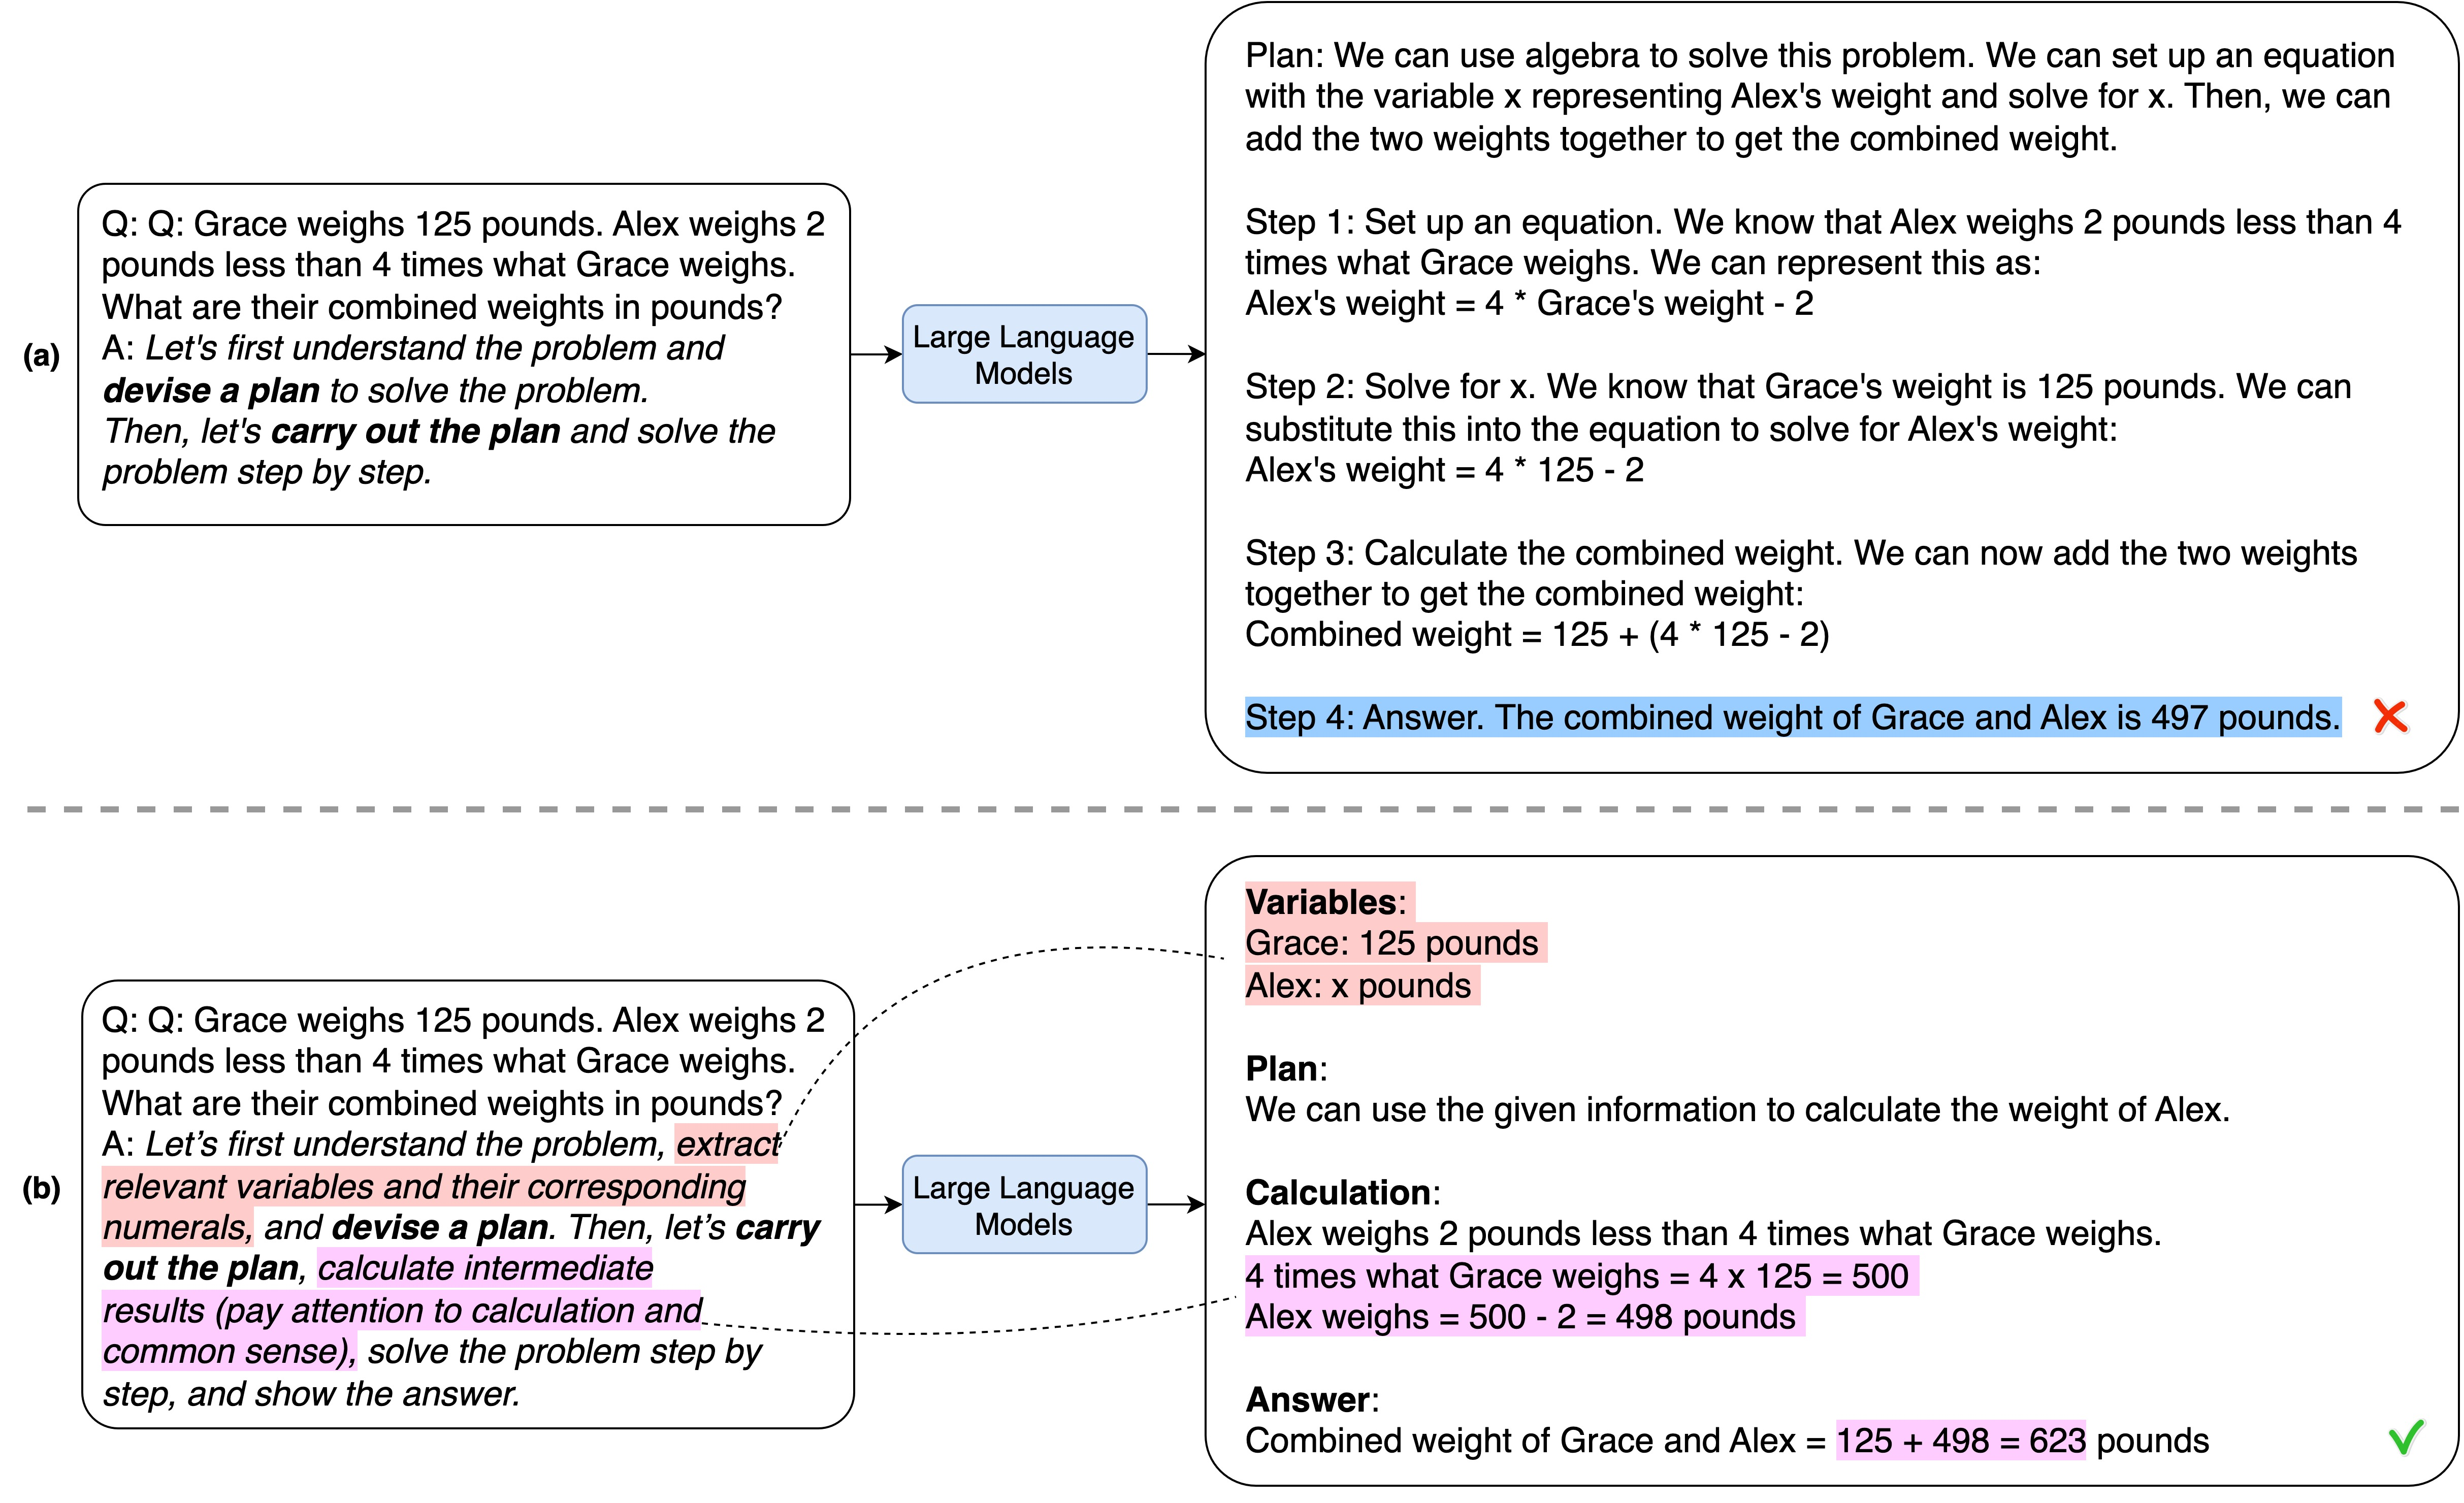
\includegraphics[width=0.8\linewidth]{math-cot-2.jpg}
    \caption{Comparison of PS prompting with PS+ prompting}
    \label{fig:enter-label}
\end{figure}
\subsection{Few-Shot Prompting}

In Few-Shot Prompting, the model is provided with a small set of examples within the prompt itself. These examples are selected to demonstrate the task or the type of response desired. By analyzing these examples, the LLM learns the context and structure of the task, allowing it to apply this understanding to new, similar problems. Few-Shot Prompting is akin to In-Context Learning (ICL), but instead of providing analogies, it furnishes the prompt with concrete examples followed by the LLM's desired answers. 

For instance, consider the following examples:
\begin{itemize}
    \item Example 1: "Emma left her keys in the freezer. Why? - Emma was carrying a lot of things and absent-mindedly put her keys in the freezer."
    \item Example 2: "Mike found his phone in the bathroom cabinet. Why? - Mike was multi-tasking, cleaning the bathroom while talking on the phone, and he left it there accidentally."
\end{itemize}

Now, when the LLM is presented with the target question about John's coffee cup, it has context from these examples on how to approach and solve the problem:

\textit{Target Question with Few-Shot Learning Applied}:
\begin{quote}
    "John found his coffee cup in the refrigerator. Why was it there?"
\end{quote}
Based on the learning from the examples, the LLM might reason in the following manner:
\begin{itemize}
    \item Similar to Emma, who absent-mindedly left her keys in the freezer while being preoccupied with carrying multiple items, it is plausible that John was also engaged in multitasking.
    \item Drawing a parallel with Mike's situation, where his attention was divided, leading to him leaving his phone in the bathroom, John might have been similarly distracted.
    \item Consequently, it is reasonable to infer that John could have placed his coffee cup in the refrigerator during a moment of absent-mindedness or distraction, akin to the scenarios described in the examples.
\end{itemize}


\subsection{Recursive Prompting}

Recursive Prompting is characterized by its process of building upon the model's previous responses to develop subsequent prompts, creating a sequence of question-and-answer cycles that delve deeper into the subject matter.

In Recursive Prompting, the initial response of the model to a prompt is not the end but the starting point for further inquiry. The model's response is analyzed, and based on this, a new prompt is formulated, often seeking clarification, additional detail, or expansion on certain aspects of the initial response. This process repeats, with each iteration refining or extending the model's understanding of the topic or problem at hand.

\textbf{Example}:
\begin{enumerate}
    \item \textbf{Initial Prompt}: "Explain how photosynthesis works in plants."
    \item \textbf{LLM's Response}: "Photosynthesis in plants is a process where plants convert light energy into chemical energy. It occurs in the chloroplasts of plant cells where carbon dioxide and water are converted into glucose and oxygen using sunlight."
    \item \textbf{Recursive Prompt 1}: "What role does chlorophyll play in this process?"
    \item \textbf{LLM's Response}: "Chlorophyll, the green pigment in plants, is crucial for photosynthesis. It absorbs light, primarily blue and red wavelengths, and uses this energy to drive the chemical reactions involved in making glucose."
    \item \textbf{Recursive Prompt 2}: "Can you explain the importance of sunlight in photosynthesis?"
    \item \textbf{LLM's Response}: "Sunlight provides the energy required for photosynthesis. It powers the reaction that converts carbon dioxide and water into glucose and oxygen, which is the primary energy source for the plant."
    \item \textbf{Recursive Prompt 3}: "How do plants use the glucose produced in photosynthesis?"
    \item \textbf{LLM's Response}: "Plants use glucose as a source of energy for growth and development. It's used to make cellulose for cell walls and starch for storage. Glucose is also vital for other metabolic processes within the plant."
\end{enumerate}

\section{Datasets}
\subsection{Winograd Schema Challenge (WSC)}
A Winograd schema is a pair of sentences that differ in only one or two words and that contain an ambiguity that is resolved in opposite ways in the two sentences and requires the use of world knowledge and reasoning for its resolution. The schema takes its name from a well-known example by Terry Winograd:
\begin{quote}
    "The city councilmen refused the demonstrators a permit because they [feared/advocated] violence."
\end{quote}


If the word is feared'', then they'' presumably refers to the city council; if it is advocated'' then they'' presumably refers to the demonstrators. [9]

\subsection{HellaSwag}
HellaSWAG is a dataset for studying grounded commonsense inference. It consists of 70k multiple choice questions about grounded situations: each question comes from one of two domains -- activitynet or wikihow -- with four answer choices about what might happen next in the scene. The correct answer is the (real) sentence for the next event; the three incorrect answers are adversarially generated and human verified, so as to fool machines but not humans.[8]

\subsection{CommonsenseQA}
The CommonsenseQA is a dataset for commonsense question answering task. The dataset consists of 12,247 questions with 5 choices each. The dataset was generated by Amazon Mechanical Turk workers in the following process (an example is provided in parentheses):

\begin{enumerate}
    \item a crowd worker observes a source concept from ConceptNet (“River”) and three target concepts (“Waterfall”, “Bridge”, “Valley”) that are all related by the same ConceptNet relation (“AtLocation”),
    \item the worker authors three questions, one per target concept, such that only that particular target concept is the answer, while the other two distractor concepts are not, (“Where on a river can you hold a cup upright to catch water on a sunny day?”, “Where can I stand on a river to see water falling without getting wet?”, “I’m crossing the river, my feet are wet but my body is dry, where am I?”)
    \item for each question, another worker chooses one additional distractor from Concept Net (“pebble”, “stream”, “bank”), and the author another distractor (“mountain”, “bottom”, “island”) manually. [7]


\end{enumerate}


\section{Initial ideas}

The testing hypothesis for Few-Shot Prompting is that more examples lead to better accuracy for target questions. Similarly, deeper recursion up to a certain point provides more thorough answers...
"We intend to test these hypotheses using the (Winograd Schema Challenge (WSC)?) as our primary dataset. Our approach involves enriching target questions from the WSC with varying contexts and examples for Few-Shot Prompting, and progressively deeper inquiries for Recursive Prompting,...? The effectiveness of each strategy will be evaluated by measuring the accuracy of the LLM’s responses in relation to the number of contextual examples and the depth of recursion used in the prompts."\par

Another idea is that we investigate the efficacy of two promising prompt strategies, Chain of Thought (CoT) and Incontext Learning (ICL), in enhancing commonsense reasoning abilities using the Winograd Schema Challenge dataset as our benchmark. We preprocess the dataset to extract relevant prompts and questions, then design and implement experimental setups within pretrained LLMs. Through evaluation, we compare the performance of LLMs guided with CoT and ICL prompt strategies, focusing on metrics such as accuracy and reasoning ability. Our analysis of the results provides valuable insights into the strengths, weaknesses, and implications of each strategy.







\section{References}

[1] Banghao C., Zhaofeng Z., Nicolas L., Shengxin Z.: Unleashing the potential of prompt engineering in Large Language Models: a comprehensive review;
Dostopano na: \url{https://arxiv.org/pdf/2310.14735.pdf} [Dostopano Marec 2024]\newline

[2] Zhang Z., Zhang A. , Mu Li ,  Smola A.: AUTOMATIC CHAIN OF THOUGHT PROMPTING IN LARGE LANGUAGE MODELS;
Dostopano na: \url{https://arxiv.org/pdf/2210.03493.pdf} [Dostopano Marec 2024]\newline

[3] Zhang Z., Zhang A. , Mu Li ,  Smola A.: Auto-CoT: Automatic Chain of Thought Prompting in Large Language Models (ICLR 2023);
Dostopano na: \url{https://github.com/amazon-science/auto-cot} [Dostopano Marec 2024]\newline

[4] Qingxiu D., Lei Li , Damai D. , Ce Z. , Zhiyong W. , Baobao C. , Xu S. , Jingjing X. , Lei L.,  Zhifang S.: A Survey on In-context Learning;
Dostopano na: \url{https://arxiv.org/pdf/2301.00234.pdf} [Dostopano Marec 2024]\newline

[5] Medium: Understanding In-context Learning in Large Language Models ( like GPT3/GPT-J/GPTNeoX );
Dostopano na: \url{https://medium.com/@mlblogging.k/understanding-in-context-learning-in-large-language-models-like-gpt3-gpt-j-gptneox-e0a71063a6db} [Dostopano Marec 2024]\newline

[6] Pandey p.,  Medium: Chain of Thought Prompting: Guiding LLMs Step-by-Step;
Dostopano na: \url{https://medium.com/@pankaj_pandey/chain-of-thought-prompting-guiding-llms-step-by-step-e6eac32d02d8} [Dostopano Marec 2024]\newline

[7] Talmor et al: CommonsenseQA;
Dostopano na: \url{https://paperswithcode.com/dataset/commonsenseqa} [Dostopano Marec 2024]\newline

[8] Mosaic: HellaSwag;
Dostopano na: \url{ https://allenai.org/data/hellaswag?trk=article-ssr-frontend-pulse_little-text-block} [Dostopano Marec 2024]\newline

[9] Paperswithcode: WSC (Winograd Schema Challenge);
Dostopano na: \url{https://paperswithcode.com/dataset/wsc} [Dostopano Marec 2024]\newline

[10] Lei Wang, Wanyu Xu, Yihuai Lan, Zhiqiang Hu, Yunshi Lan, Roy Ka-Wei Lee, Ee-Peng Lim: Plan-and-Solve Prompting: Improving Zero-Shot Chain-of-Thought Reasoning by Large Language Models; 
Dostopano na: \url{https://doi.org/10.48550/arXiv.2305.04091} [Dostopano Marec 2024] \newline

\end{document}